\section{Диффузия легирующей примеси}

Приконтактные области выполняют роль резервуаров электронов. Они сильно легированы. Концентрация донорной примеси в них $N_{D} = 10^{24}\,m^{-3}$. В случае РТГС, представленной на рис.~\ref{fig:RTHSModel} на основе $AlGaAs$ в роли донорной примеси выступает $Si$.

\begin{figure}[h!]
	\centering
	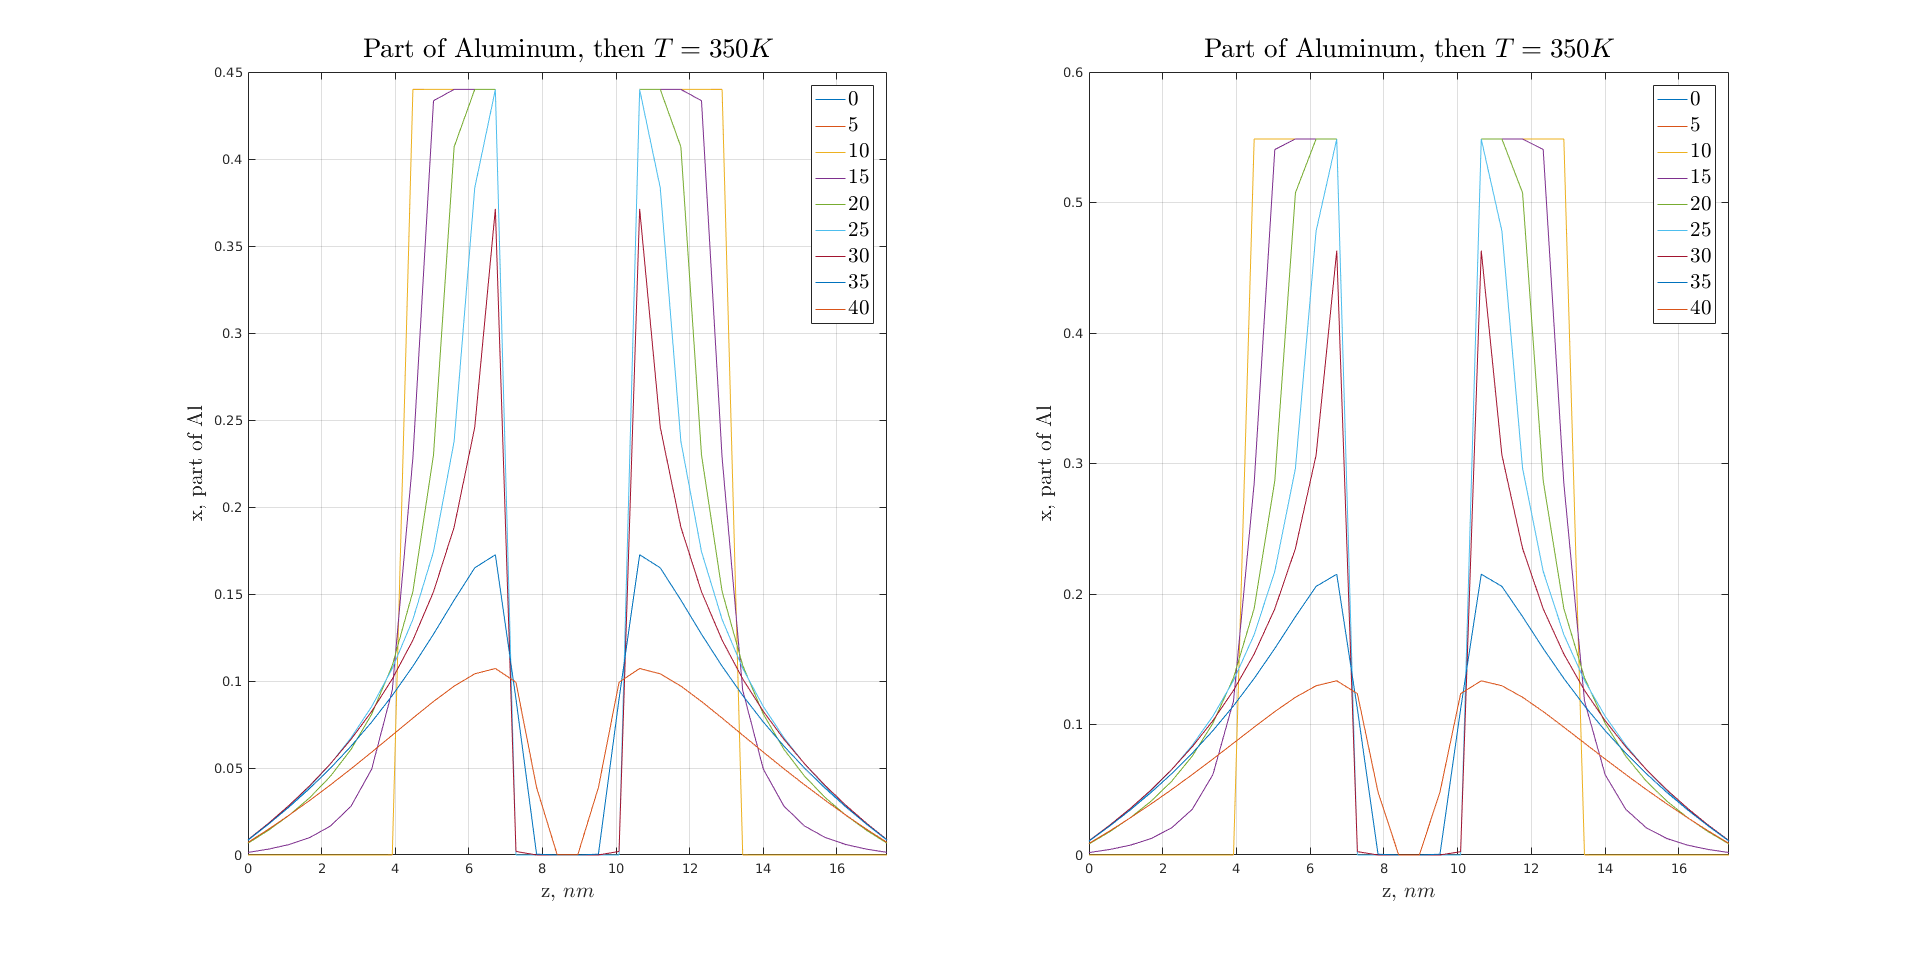
\includegraphics[width=\linewidth]{DAlGaAs_Si}
	\caption{Расплытие потенциального рельефа $Al_{x}Ga_{1−x}As$ и Si из приконтактных областей} 
	\label{fig:DAlGaAs_Si}
\end{figure}

\begin{figure}[h!]
	\centering
	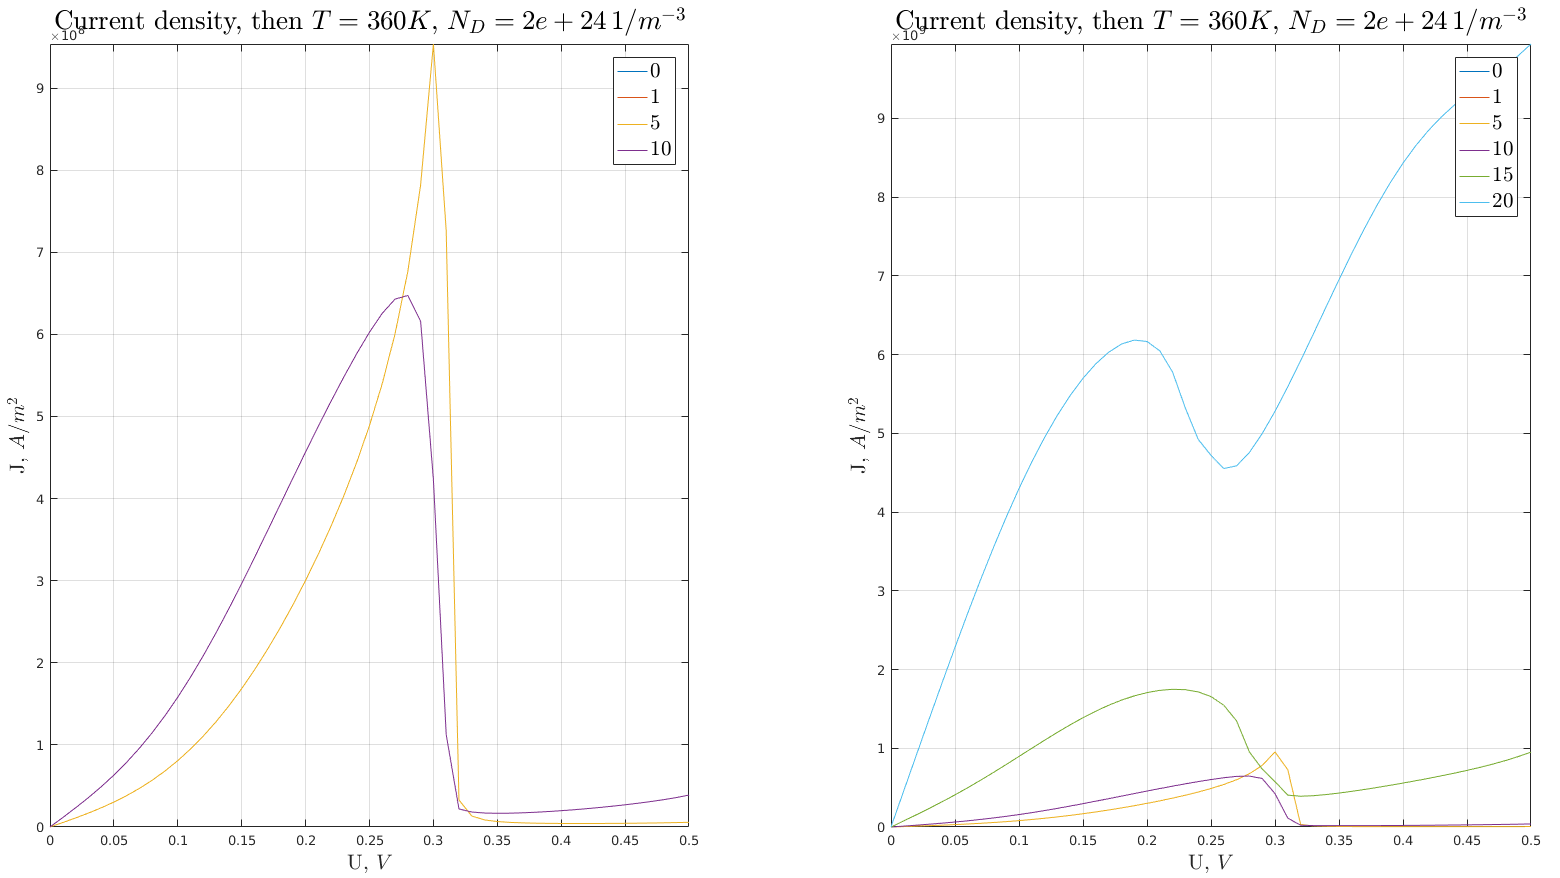
\includegraphics[width=\linewidth]{JDAlGaAs_Si}
	\caption{Деградация тока через РГТС}
	\label{fig:JDAlGaAs_Si}
\end{figure}

Повышение температуры на $60$ приводит к значительной деградации, причем в первые 5 лет деградации подвержены спейсеры, которые предохраняют РТГС от деградации ВАХ, в соответствии с результатами полученными ранее.